A toy model of AOD provides a simple-to-understand representation for how real and Monte Carlo simulated data will react under optimization conditions for derivation production jobs. 
One commonality between both data and MC is the branch data within both is made of a mixture between repeated integer-like data and randomized floating-point data (i.e. data that has both easily and difficult to compress.)
Replicating this mixture of data in a branch would give us an effective model that would resemble how current derivation jobs would act on real and MC simulated data. 
These toy model mixtures would provide an avenue to test opportunities for optimizing the demand on the GRID by first looking at limiting basket sizes and their effects on compression of branches. 

\section{Introducing the Toy Model}

There were a number of iterations to the toy model, but the first was constructed by filling up a TTree with branches that each have vectors with varying number of random floats written and read back.
This original model had four distinct branches, each with a set number of events ($N=1000$), and each event having a number of entries, vectors with 1, 10, 100, and 1000 floats each.
Specifics are illustrated in Appendix \ref{appendix:toy_model_no_mix_code}.

% How we compressed these was through calling AutoFlush
Once the branches were filled, ROOT then will loop over each of the branches in the TTree and at regular intervals will remove the baskets from memory, compress, and write the baskets to disk (flushed), as was discussed in Section $\S \ref{section: ATLASIO_TTreeObject}$.
%  the compression factor for each branch that was filled.
To reiterate, the goal was to create branches with data similar to what could be found in real post-reconstructed data samples.
This would mean creating for branches with compression ratios on the order $\mathcal{O}(5)$, as is typical for such real data. 


\section{Toy Model Compression}

\subsection{All Random Float Branches}

Upon reading back the ROOT file, the user would be able to see the original size of the file (Total-file-size), the compressed file size (File-size), the number of baskets per branch, the basket size, and other information. 
Since the branches had vectors with exclusively random floats, it becomes apparent that the more randomization in the branches the harder it is to compress. 

\begin{figure}[h]
    \caption{Compression factors of $N=1000$ entries per branch with random-valued vectors of varying size.}
    \label{fig:toymodel_compF_rndm_vectors}
    \centering
    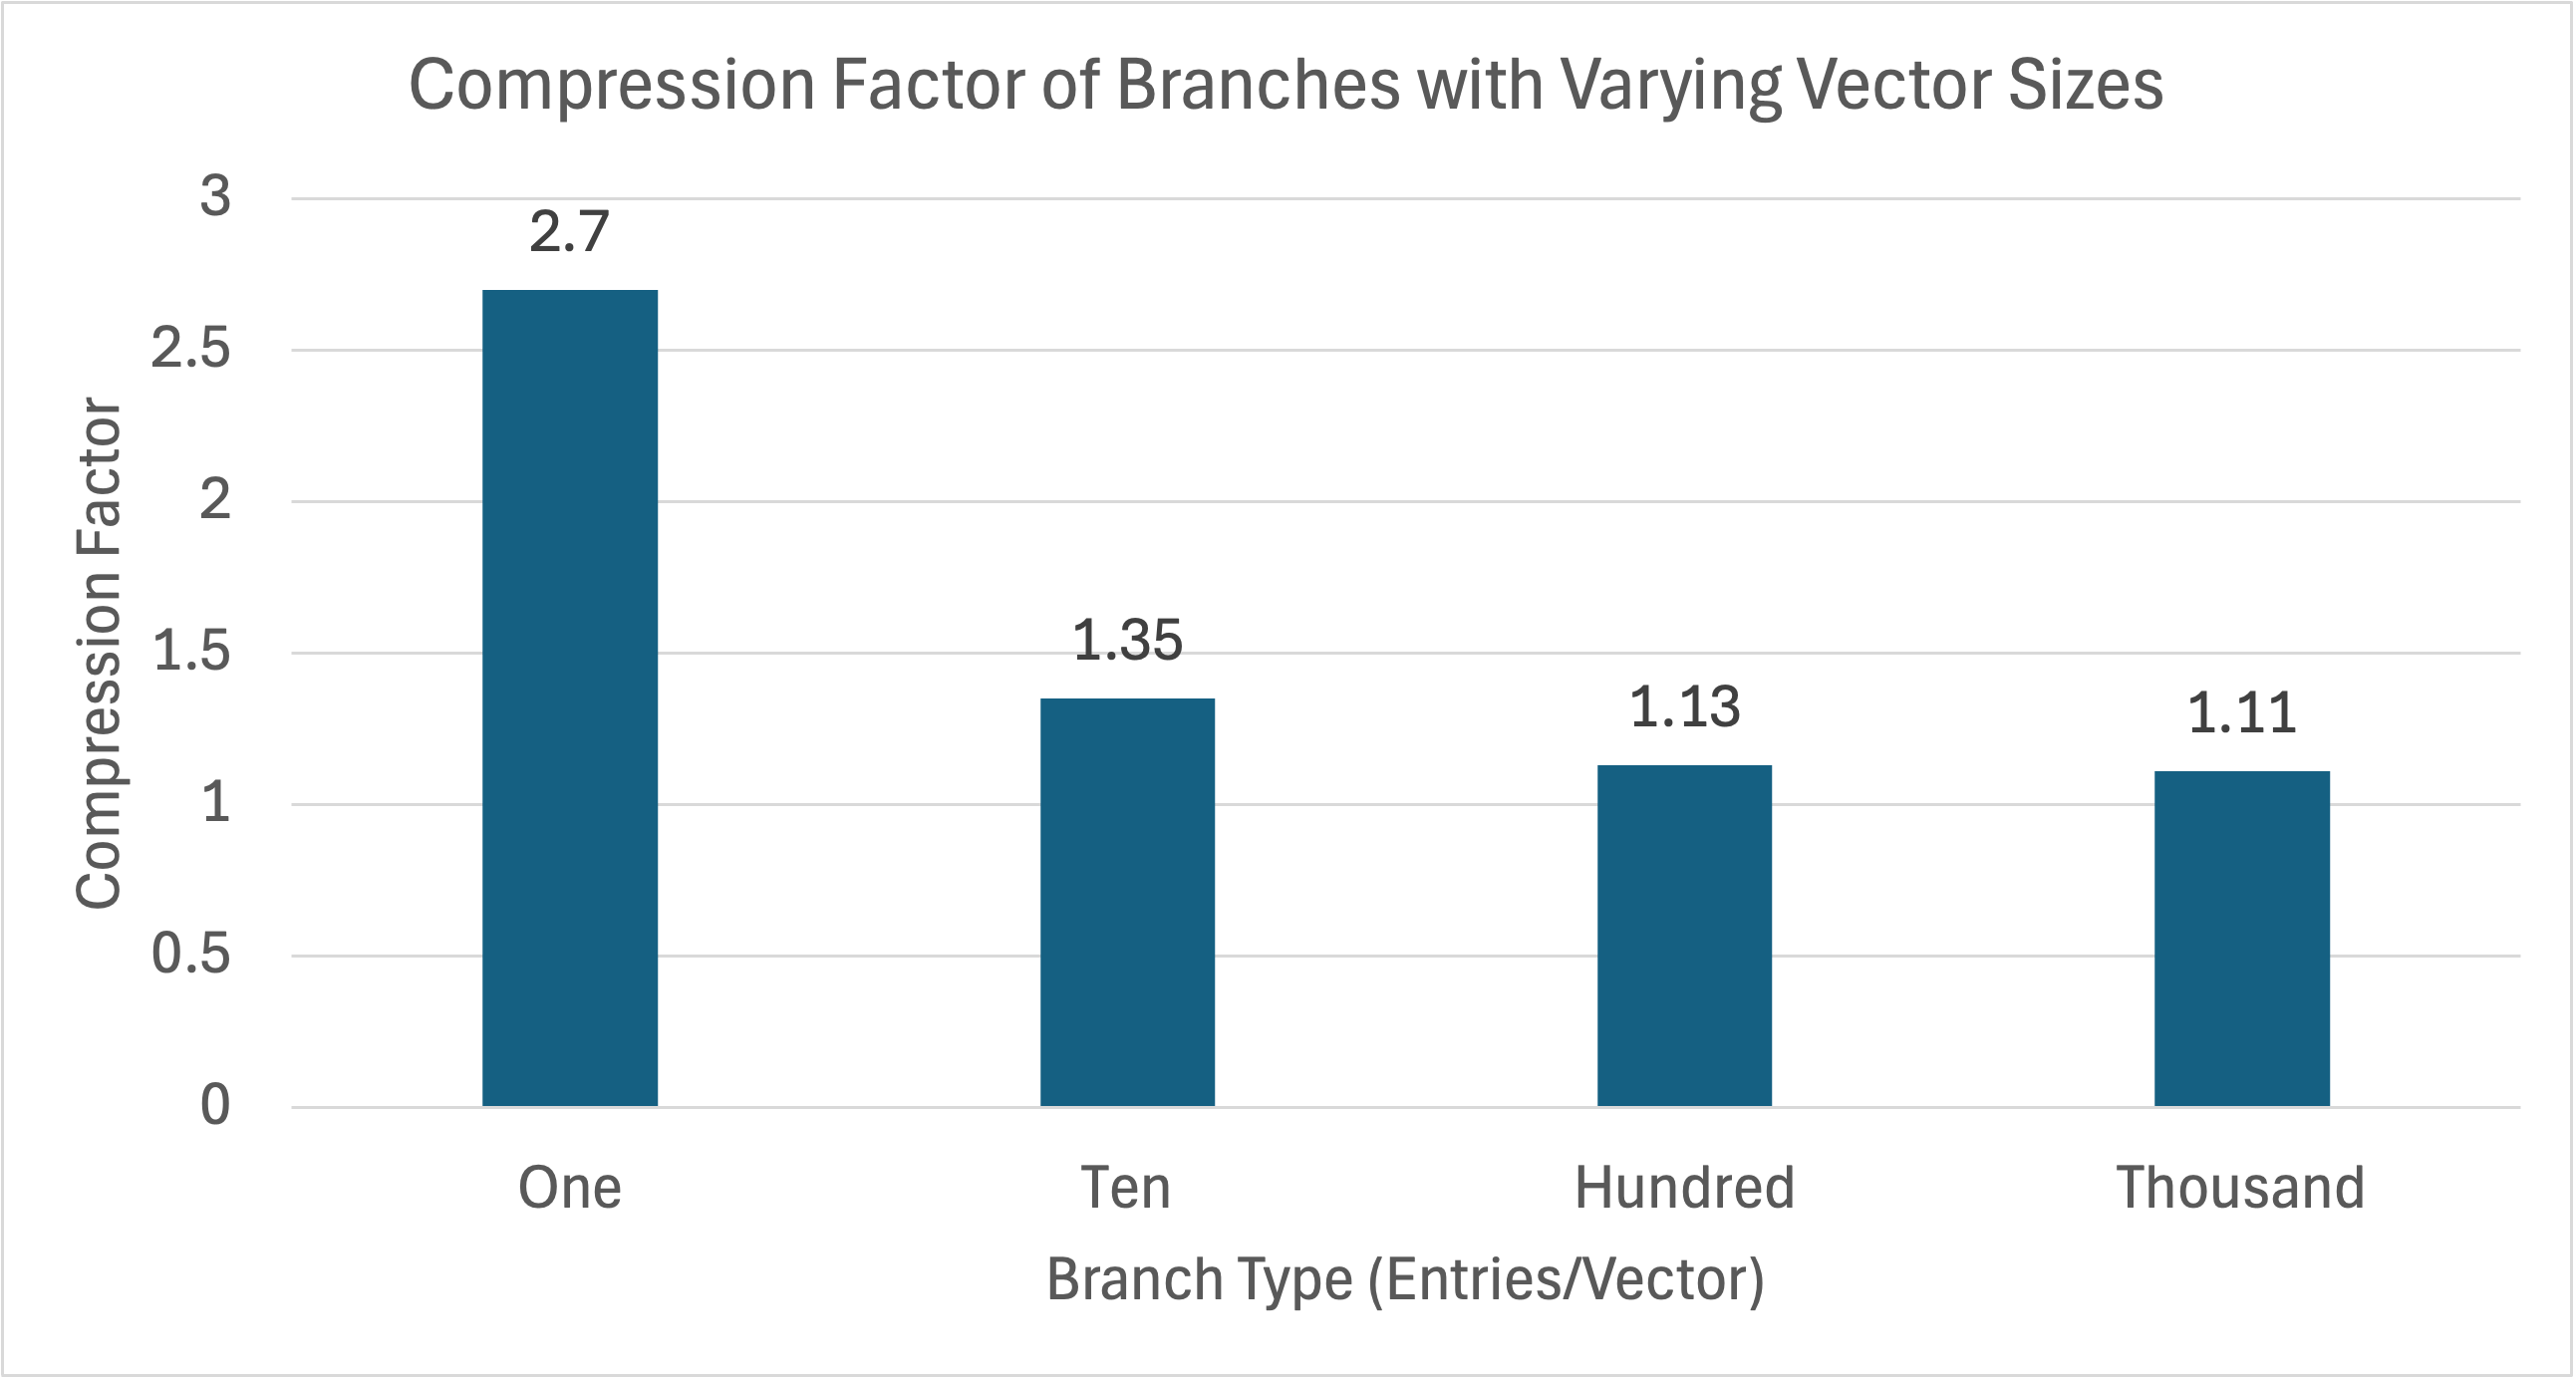
\includegraphics[width=.8\textwidth]{content/toymodel_content/branch_compfacts_nomix.png}
\end{figure}

% \begin{figure}[h]
%     \caption{File size of $N=1000$ entries per branch with random-valued vectors of varying size.}
%     \label{fig:toymodel_filesize_rndm_vectors}
%     \centering
%     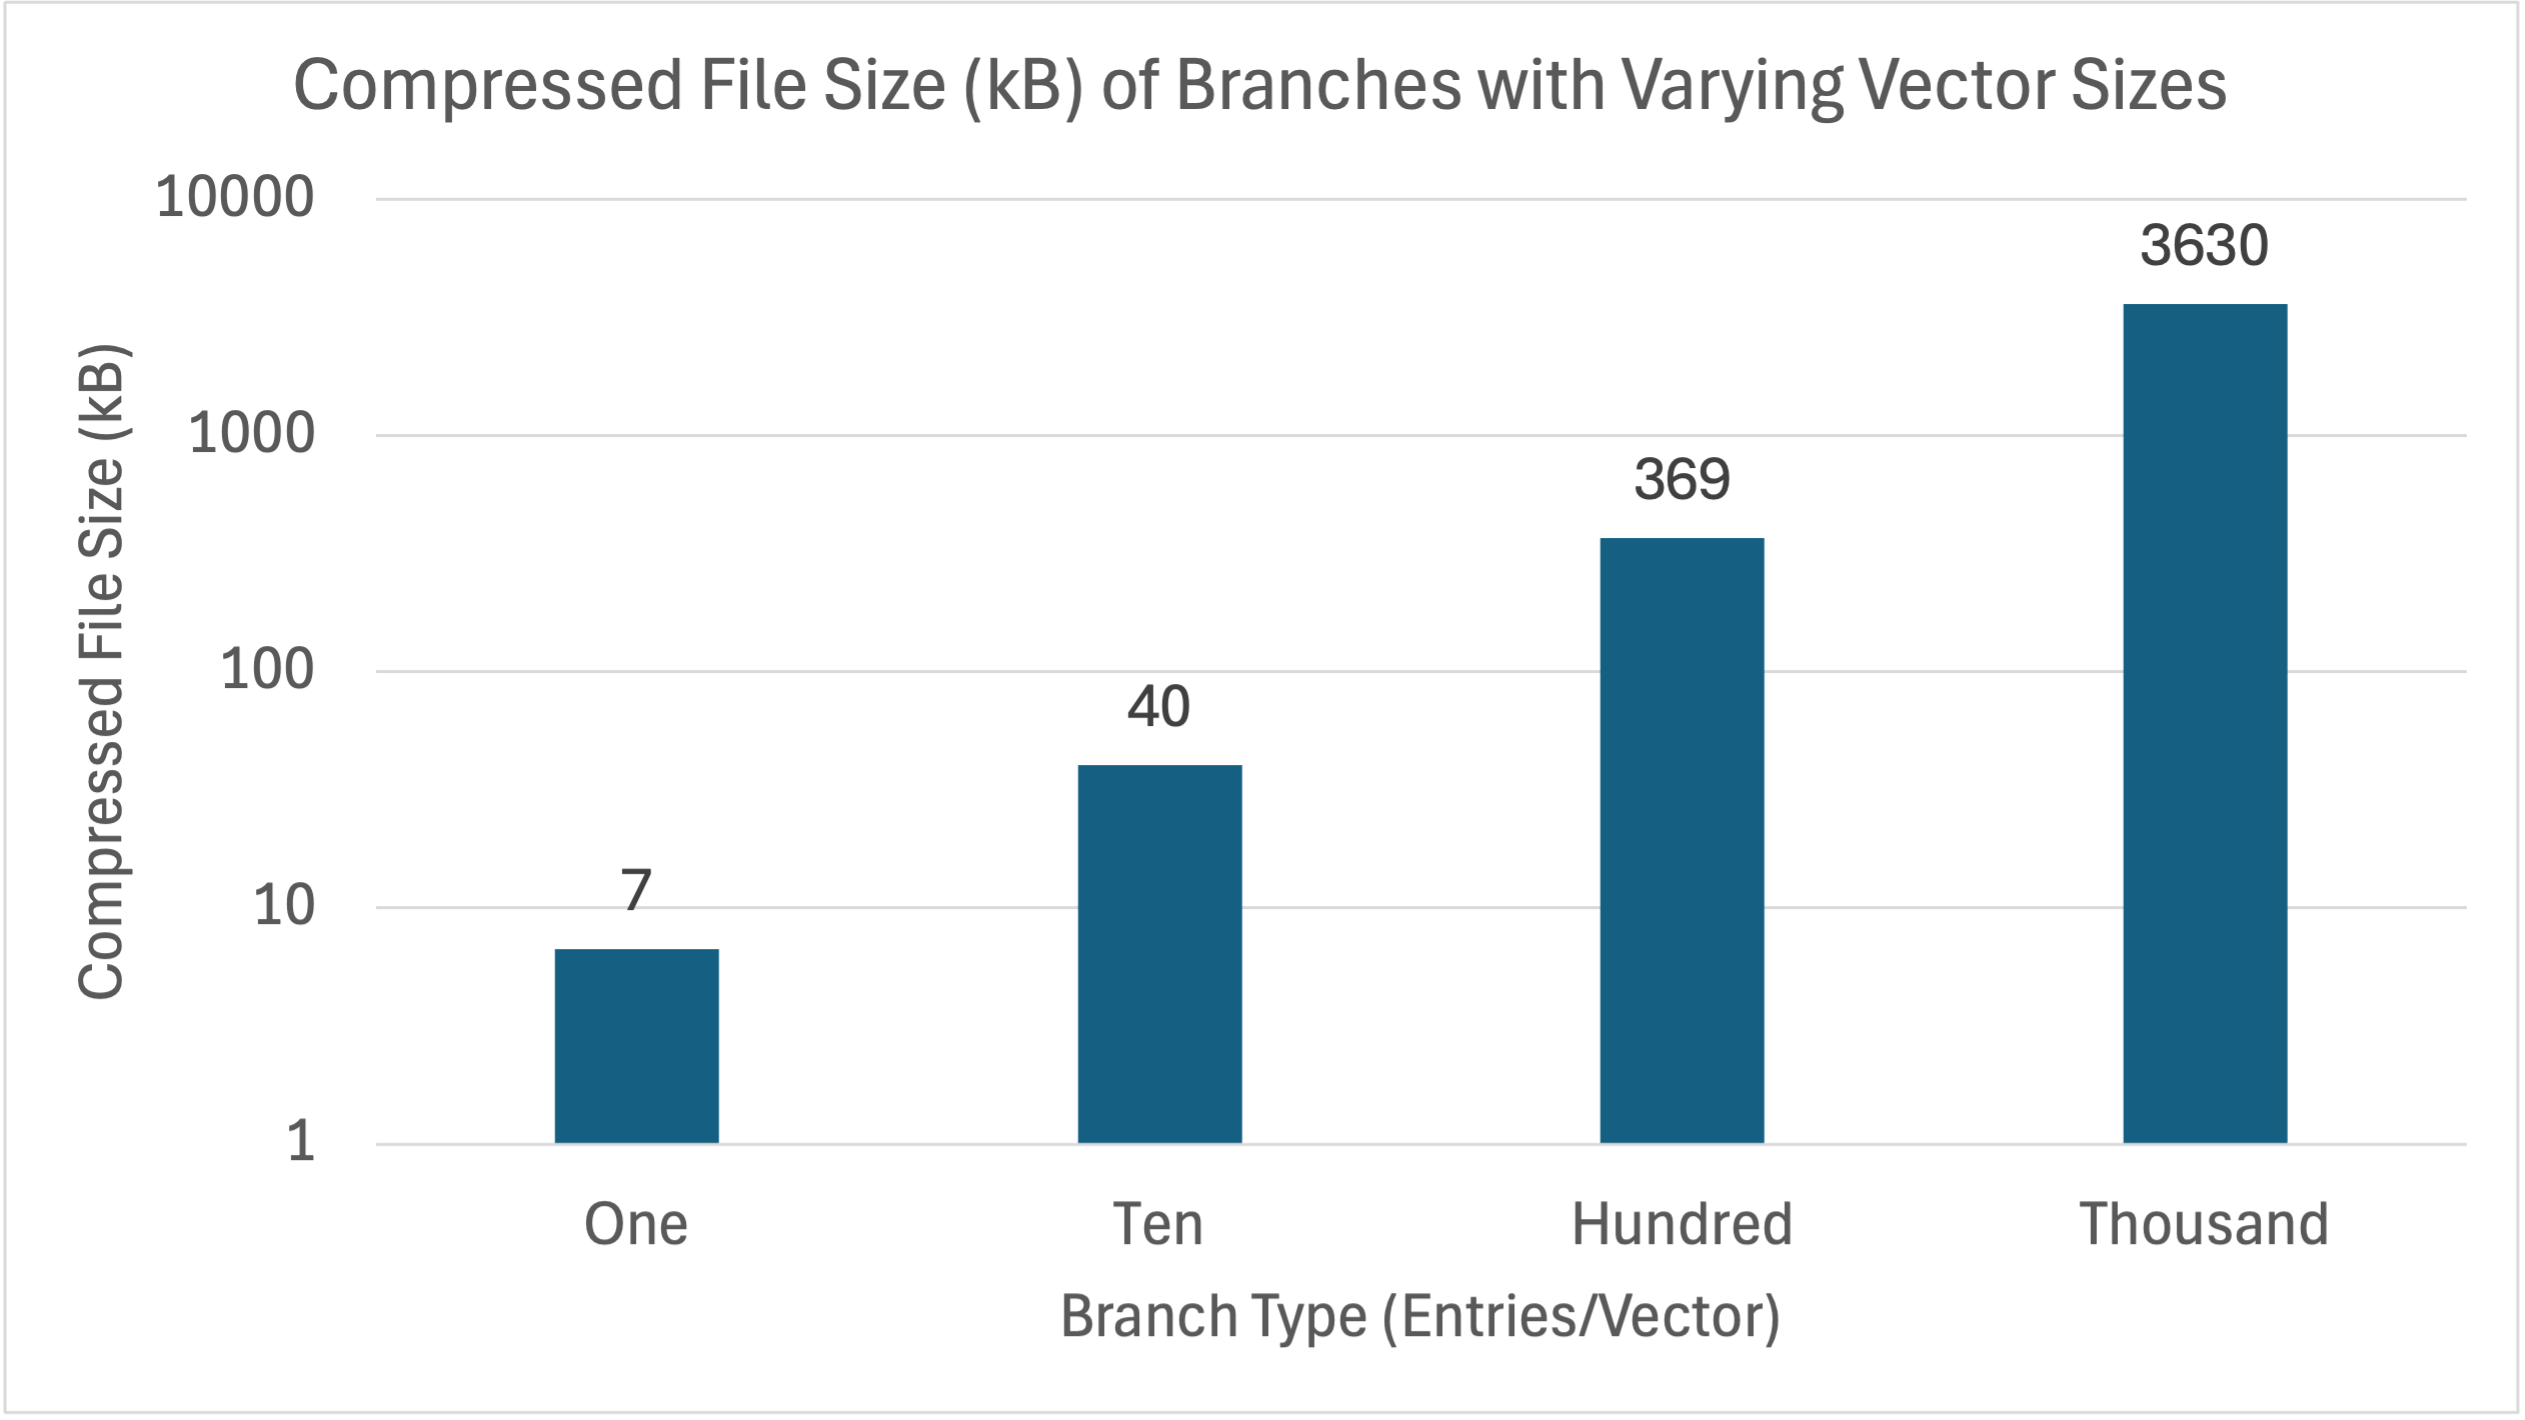
\includegraphics[width=.8\textwidth]{content/toymodel_content/branch_fileSize_nomix.png}
% \end{figure}

Figure \ref{fig:toymodel_compF_rndm_vectors} shows compression drop-off as the branches with more randomized floats per vector were present.
This is the leading indication that there needs to be more compressible data within the branches. 

\subsection{Mixed-Random Float Branches}
The branches needed to have some balance between compressible and incompressible data to mimic the compression ratio found in real data.
How this was achieved was by filling each vector with different ratios of random floats and repeating integers, see Appendix \ref{appendix:toy_model_WITH_mix_code}.
